% Формат бумаги: А4.
\documentclass[a4paper]{report}
\usepackage[utf8]{inputenc}
\usepackage[russian]{babel}
\usepackage{amsmath,amsfonts,amssymb,cite,url,verbatim,graphicx,wrapfig}
\graphicspath{{images/}}
\usepackage{booktabs}
\usepackage{graphicx}
\usepackage{array}
\usepackage{relsize}
\usepackage{algorithm2e}



\SetKwInput{KwData}{Вход}
\SetKwInput{KwResult}{Выход}
\SetKwInput{KwIn}{Входные данные}
\SetKwInput{KwOut}{Выходные данные}
\SetKwIF{If}{ElseIf}{Else}{если}{тогда}{иначе если}{иначе}{конец условия}
\SetKwFor{While}{до тех пор, пока}{выполнять}{конец цикла}
\SetKw{KwTo}{от}
\SetKw{KwRet}{возвратить}
\SetKw{Return}{возвратить}
\SetKwBlock{Begin}{начало блока}{конец блока}
\SetKwSwitch{Switch}{Case}{Other}{Проверить значение}{и выполнить}{вариант}{в противном случае}{конец варианта}{конец проверки значений}
\SetKwFor{For}{цикл}{выполнять}{конец цикла}
\SetKwFor{ForEach}{для всех}{}{}
\SetKwRepeat{Repeat}{повторять}{до тех пор, пока}
\SetAlgorithmName{Алгоритм}{алгоритм}{Список алгоритмов}


% Поля: верхнее – 2 см, нижнее – 2 см, левое – 3 см, правое – 1.5 см.
\usepackage{geometry}
\geometry{
	left = 3cm,
	top = 2cm,
	right = 1.5cm,
	bottom = 2cm
}


%\setlength{\parindent}{1.5cm}

% Кегль: основной текст – 14 пт, названия параграфов – 16 пт, названия глав – 18 пт, текст в таблице, подписи к рисункам, таблицам – 12 пт.
\renewcommand{\small}{\fontsize{12}{12}\selectfont}
\renewcommand{\normalsize}{\fontsize{14}{14}\selectfont}
\renewcommand{\large}{\fontsize{16}{16}\selectfont}
\renewcommand{\Large}{\fontsize{18}{18}\selectfont}
\renewcommand{\huge}{\fontsize{20}{20}\selectfont}
\usepackage{sectsty}
\sectionfont{\Large}
\subsectionfont{\large}
\paragraphfont{\normalsize}
\usepackage[font=small]{caption}

% Межстрочный интервал: 1.5 строки.
\usepackage{setspace}
\linespread{1.5}

% Абзацный отступ. Первая строка каждого абзаца должна иметь абзацный отступ 1.25 см.
\usepackage{indentfirst}
\setlength{\parindent}{1.25cm}

% Выравнивание основного текста по ширине поля.
\usepackage{ragged2e}
\justifying

%%% здесь лучше ничего не трогать
\setcounter{tocdepth}{2}
\renewcommand{\thesection}{}
\renewcommand{\thesubsection}{}
\allsectionsfont{\centering}
\usepackage{titlesec}
\newcommand{\sectionbreak}{\clearpage}
\usepackage{tocloft}
\cftsetindents{section}{0em}{0em}
\cftsetindents{subsection}{2em}{0em}
\AtBeginDocument{\renewcommand{\contentsname}{\begin{center} \vskip-2.5cm \Large{Содержание} \end{center}}}
\AtBeginDocument{\renewcommand{\bibname}{}}
%%%

\begin{document}
	%%%%% TITLE PAGE %%%%%
\thispagestyle{empty}
\begin{center}
\textsc{Санкт-Петербургский государственный университет \\
\textbf{Кафедра технологии программирования}} \\ 
\vspace{3cm} 
\Large{\textbf{Башарин Егор Валерьевич}} \\
\vspace{1.5cm}
\large{\textbf{Выпускная квалификационная работа бакалавра}} \\ 
\vspace{2.5cm}
\Large{\textbf{Контекстная обработка данных социальных сетей}} \\ 
\normalsize{Направление 010400 \\
Прикладная математика и информатика} \\
\end{center}
\vspace{2.5cm}
\hspace{9cm} Научный руководитель, \\
\hspace*{9cm} старший преподаватель \\
\hspace*{9cm} Попова С.В. 
\begin{center}
\vfill
Санкт-Петербург \\
2016
\end{center}
	\newpage
	
	%%%%% CONTENTS %%%%%
	\tableofcontents
	\newpage
	
	
%%%%%%%%%%%%%%%%%%%%%%%%%%%%%%%%%%%%%%%%%%%%%%%%%%%%%%%
%%%%%%%%%%%%%%%%%%%%%%%%%%%%%%%%%%%%%%%%%%%%%%%%%%%%%%%
                   %%%%% Intro %%%%%
%%%%%%%%%%%%%%%%%%%%%%%%%%%%%%%%%%%%%%%%%%%%%%%%%%%%%%%
%%%%%%%%%%%%%%%%%%%%%%%%%%%%%%%%%%%%%%%%%%%%%%%%%%%%%%%
	\section{Введение} 
	В настоящее время явление социальных сетей достаточно распространено. Социальные сети уверенно вошли в жизнь современного человека и теперь занимают в ней значимую часть. Главным образом они оказывают влияние на поведение, предубеждения, ценности и намерения человека, что отражается во всех сферах его деятельности. Оказываемое влияние, быстрый рост популярности и открытый доступ к контенту привлекли к~социальным сетям внимание правительства, финансовых организаций и~исследователей. 
	Выделение ключевых концепций стало важным условием для порождения знаний и формулирования стратегий.
	 Анализ полученных данных помогает исследователям улучшить понимание об информационных потоках, о формировании и распространении мнений, о~связи ценностей и предубеждений пользователя и генерируемого им контента. 
	 
	Существенным барьером при использовании социальных сетей является необходимость выбора методологии для сбора, обработки и анализа информации, полученной с сайтов социальных сетей. Однако, существуют компании по производству программного обеспечения, разрабатывающие проприетарные системы сбора информации для визуализации данных, и~исследователи, занимающиеся разработкой экспертных систем для анализа настроений \cite{bib:Kaklauskas}. 
	
Пользователи социальных сетей ежедневно публикуют данные о своей активности, чувствах и мыслях, выражая свое мнение и позицию. Это способствует появлению в социальных сетях групп пользователей (сообществ), имеющих общие интересы. Для выявления ключевых концепций и~ тематик присущих группе пользователей используется контекстная обработка  генерируемого ими контента. В данной работе контекстная обработка данных основана на идеях и принципах тематического моделирования. Результаты такой обработки могут использоваться для мониторинга мнений и политических взглядов пользователей или для предсказания поведения рынка. \\

%%%%%%%%%%%%%%%%%%%%%%%%%%%%%%%%%%%%%%%%%%%%%%%%%%%%%%%
%%%%%%%%%%%%%%%%%%%%%%%%%%%%%%%%%%%%%%%%%%%%%%%%%%%%%%%
                   %%%%% Постановка задачи %%%%%
%%%%%%%%%%%%%%%%%%%%%%%%%%%%%%%%%%%%%%%%%%%%%%%%%%%%%%%
%%%%%%%%%%%%%%%%%%%%%%%%%%%%%%%%%%%%%%%%%%%%%%%%%%%%%%%
	 
	\section{Постановка задачи}
	Целью данной работы является изучение методов контекстной обработки данных социальных сетей, в основе которых лежат принципы и идеи тематического моделирования. Под социальной сетью понимается веб-сайт или онлайн-сервис, который предназначен для поддержания социальных взаимоотношений при помощи Интернета. 
	
	 Для того чтобы достичь поставленной цели предлагается выполнить следующий ряд задач:
	
	
	\renewcommand{\labelenumi}{\arabic{enumi}.}
	\renewcommand{\labelenumii}{\arabic{enumi}.\arabic{enumii}}

	\begin{enumerate}
	\item{Выбор источника данных}
		%\begin{enumerate}
		%\item{Обзор социальных сетей}
		%\item{Выбор социальной сети}
		%\end{enumerate}
	\item{Загрузка и предварительная обработка данных}
		%\begin{enumerate}
		%\item{Загрузка данных с веб-страниц социальной сети}
		%\item{Предварительная обработка данных}
		%\item{Разбиение данных на обучающую и тестовую части}
		%\end{enumerate}
	\item{Выбор тематической модели}
		%\begin{enumerate}
		%\item{Анализ тематических моделей}
		%\item{Выбор подходящей тематической модели}
		%\end{enumerate}
	\item{Построение тематической модели}
		%\begin{enumerate}
		%\item{Выбор метода для оценивания параметров тематической модели}
		%\item{Реализация алгоритма для построения тематической модели}
		%\item{Обучение тематической модели}
		%\end{enumerate}
	\item{Оценка качества модели}
		%\begin{enumerate}
		%\item{Обзор и анализ оценок качества тематических моделей}
		%\item{Оценка качества построенной модели}
		%\end{enumerate}
	%\item{Анализ полученных результатов}
	\end{enumerate}

%%%%%%%%%%%%%%%%%%%%%%%%%%%%%%%%%%%%%%%%%%%%%%%%%%%%%%%
%%%%%%%%%%%%%%%%%%%%%%%%%%%%%%%%%%%%%%%%%%%%%%%%%%%%%%%
                   %%%%% Обзор литературы %%%%%
%%%%%%%%%%%%%%%%%%%%%%%%%%%%%%%%%%%%%%%%%%%%%%%%%%%%%%%
%%%%%%%%%%%%%%%%%%%%%%%%%%%%%%%%%%%%%%%%%%%%%%%%%%%%%%%
	\section{Обзор литературы}
	
	Тема данной работы тесно пересекается с информационным поиском, основы которого подробно рассмотрены в книге Кристофера Майнинга <<Introduction to Information Retrieval>> \cite{bib:InformationRetrieval}. Особое внимание стоит уделить главам 2 и 18. В главе~2 описываются методы подготовки и предварительной обработки текстовой информации. Глава~18 сосредотачивает внимание на подходах латентно-семантического анализа, который является ценным инструментом в тематическом моделировании. В конце каждой главы приведены ссылки на литературу для более подробного изучения темы. 
	
	Вероятностное латентно-семантическое моделирование стало логичным продолжением идей латентно-семантического моделирования и нашло свое применение в тематическом моделировании. Это стало причиной появления вероятностных тематических моделей. Основные принципы вероятностного латентно-семантического анализа (probabilistic latent semantic analysis - pLSA) были описаны Томасом Хоффманом в 1999 году в статье \cite{bib:Hoffman}. Затем они были развиты Дэвидом Блеем в его статье 2003 года \cite{bib:Blei}, в которой была введена и рассмотрена тематическая модель латентного размещения Дирихле (latent dirichlet allocation - LDA). Статья Д.Блея описывает основные преимущества LDA перед pLSA, а также методы построения и оценки качества тематической модели LDA. В статье Д.Блея 2012 года \cite{bib:Blei2} рассматриваются связь LDA с другими вероятностными тематическими моделями, а также применение LDA в тематическом моделировании.
	
	В техническом отчете Грегора Хейнрича <<Parameter estimation for text analysis>> \cite{bib:Heinrich}  рассматриваются методы оценки параметров моделей для тематического анализа текстов. В отчете подробно разобраны темы, связанные с основными подходами оценки параметров, сопряженными распределениями и Байесовскими сетями, а также применение данных тем для построения тематической модели LDA. 
	
	 Среди русскоязычной литературы следует обратить внимание на работы К.~В.~Воронцова.  В работе \cite{bib:Voron1} подробно описаны основные идеи вероятностного тематического моделирования. В первой части данной работы ставится задача тематического моделирования. Далее рассматриваются основные вероятностные тематические модели pLSA, LDA и их модифицированные версии, а также методы их построения и оценки.
	

	
	
	
	\section{Глава 1. Подготовка данных}
	\subsection{1.1 Обзор социальных сетей}
	
	
	
	Несмотря на то, что социальные сети появлись около 20 лет назад, их популярность растет с каждым годом. На рисунке \ref{fig:popularity}  показан график, отображающий рост числа пользоватлей социальных сетей во всем мире. По итогам 2015 года число пользователей социальных сетей превысило отметку в 2 миллиарда человек, и по прогнозам их количество будет только расти \cite{bib:Popularity}. Поэтому можно сделать вывод, что социальные сети прочно укрепляются в жизни современного человека, а их изучение становится актуальной проблемой.
	\newline
	\begin{figure}[h]
		
		\centering
		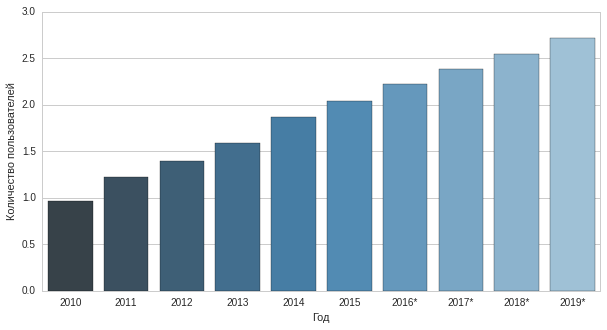
\includegraphics[width=400px]
		{imgs/Popularity.png}
		\caption{Число пользователей социальных сетей по годам}
		\label{fig:popularity}
	\end{figure}
	\newline			
	
	Число социальных сетей довольно велико, и каждая из них предоставляет различные возможности для пользователей и преследует различные цели.  На рисунке \ref{fig:stat} представлен график, отражающий количество активных пользователей в самых популярных социальных сетях на апрель 2016~года  \cite{bib:PopularNetwork}. На графике видно, что такие социальные сети как Facebook, WhatsApp, Facebook messenger и QQ пользуются наибольшей популярностью у пользователей. 	
	Также стоит обратить внимание на социальную сеть VKontakte, которая довольно популярна в российском сегменте интернета и насчитывает около 100 миллионов активных пользователей.
	
	Социальные сети Facebook и VKontakte предоставляют cхожие возможности своим пользователям: создание профиля с фотографией и информацией о себе, обмен сообщениями с другими пользователями, создание сообществ, публикация сообщений на страницах других пользователей или сообществ, загрузка видеозаписей и фотографий и множество других функций для взаимодействия между пользователями. 
	Такие социальные сети как WhatsApp, QQ, WeChat, Skype, Viber, Telegram в основном выполняют роль мессенджеров, и их предназначенение ограничивается обменом текстовой, аудио- и видео- информацией между пользователями. 
	Социальная сеть Instagram ориентирована на публикацию пользователями фотографий и видеозаписей.
	%предоставляет своим пользователям возможности обмена фотографиями и видеозаписями. 
	Особенность социальной сети Twitter - это возможность публикации коротких сообщений. LinkedIn представляет собой социальную сеть для поиска и установления деловых связей.
	
	
	
	
	


	
	\begin{figure}
		\centering
		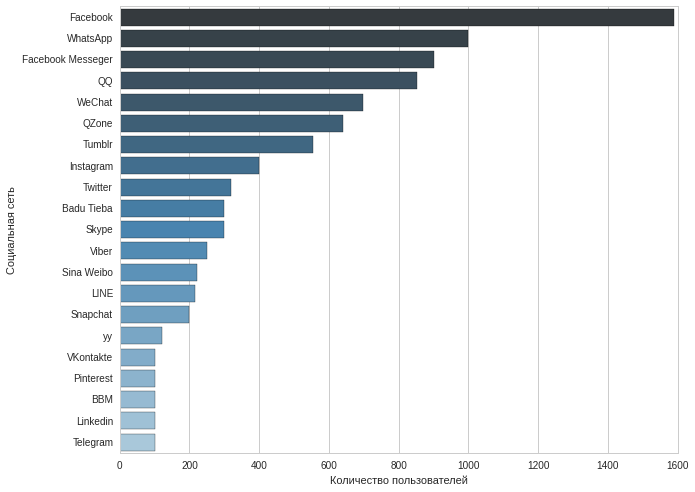
\includegraphics[width=400px]
		{imgs/NetworkStatistics.png}
		\caption{Рейтинг самых популярных  социальных сетей на апрель 2016 года}
		\label{fig:stat}
	\end{figure}
	
	
	
	
	
	\subsection{1.2 Выбор социальной сети и загрузка данных}
	
	В качестве исходных данных рассмотрим публикации в сообществах социальных сетей. 
	Такие сообщества, как правило, представляют собой одну или несколько веб-страниц. 
	Каждое сообщество обладает определенной тематической направленностью: спорт, музыка, политика, финансы и~др.
	Возможность создания сообществ поддерживается такими социальными сетями как Facebook и VKontakte. 
	В данной работе рассматривается социальная сеть VKontakte, так как она наиболее популярна в российском сегменте интернета.
			
	
	Для загрузки публикации из сообществ социальной сети VKontakte реализован программный модуль на языке программирования Python~2.7. 
	Для получения доступа к информации о сообществах и их публикациям использовалась технология API~VKontakte \cite{bib:vkapi}, которая предоставляет методы для работы с данными социальной сети \cite{bib:methods}. Число обращений к методам API имеет ограничение: не более 3 раз в секунду.
	
	API (Application programming interface, интерфейс программирования приложений) представляет собой набор готовых классов, функций и структур, предоставляемых сервисом для использования во внешних программных продуктах. 
	
	\setlength\extrarowheight{5pt}
\begin{table}[h]
\centering
\begin{tabular}{|c|c|}
\hline
\textbf{Идентификатор категории} & \textbf{Название категории} \\  \hline 
0 & Рекомендации \\ \hline
1 & Новости \\ \hline
2 & Спорт \\ \hline
3 & Музыка \\ \hline
4 & Развлечения \\ \hline
6 & Бренды \\ \hline
7 & Наука \\ \hline
8 & Культура и искусство \\ \hline
9 & Радио и телевидение \\ \hline
10 & Игры и киберспорт \\ \hline
11 & Магазины \\ \hline
12 & Красота и стиль \\ \hline
13 & Автомобили \\ \hline
\end{tabular}
\caption{Категории сообществ VKontakte}
\label{table1}
\end{table}
	
	Для загрузки данных программный модуль отправляет запросы методам API VKontakte для выполнения следующих задач:
	
	%\renewcommand{\labelenumi}{\arabic{enumi}.}
	%\renewcommand{\labelenumii}{\arabic{enumi}.\arabic{enumii}}
	\begin{enumerate}
	\item{Получение информации о категориях сообществ с помощью метода API \textit{groups.getCatalogInfo};}
	\item{Получение списка популярных сообществ для каждой категории с помощью метода API \textit{groups.getCatalog};}
	\item{Получение публикаций для каждого сообщества с помощью метода API \textit{wall.get}.}
	
	\end{enumerate}
	
	
	Информация о полученных категориях сообществ представлена в таблице \ref{table1}. Из таблицы видно, что все сообщества социальной сети делятся на 13 категорий. Для дальнейшей работы из них были выбраны 5 категорий: <<Новости>>, <<Спорт>>, <<Музыка>>, <<Развлечения>> и <<Бренды>>. Для каждой из выбранных категорий получен список популярных сообществ. Количество сообществ в каждой из категорий отображено на графике, представленном на рисунке \ref{fig:groupincat}. Общее число сообществ, для которых была получена информация, равняется 145. 
		\begin{figure}[h]
		\centering
		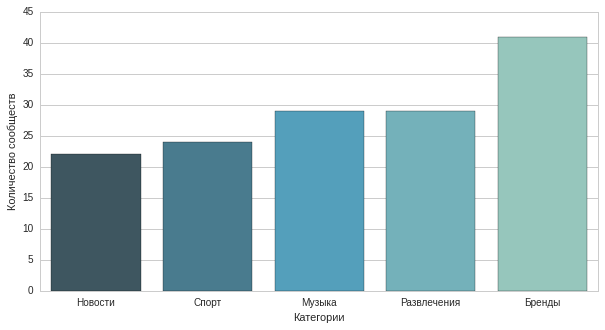
\includegraphics[width=400px]
		{imgs/GroupInCat.png}
		\caption{Количество сообществ в категориях}
		\label{fig:groupincat}
	\end{figure} 
	
	На последнем этапе работы программного модуля выполняется получение текстов всех публикаций из выбранных сообществ. На рисунке \ref{fig:numart} изображен график, показывающий число публикаций в каждой категории. 
	Общий размер загруженных данных составляет около 13~ГБ. 
	График, изображенный на рисунке \ref{fig:sizecat}, отражает объем занимаемой памяти для каждой из категорий. 
	
	
	\begin{figure}[h]
		\centering
		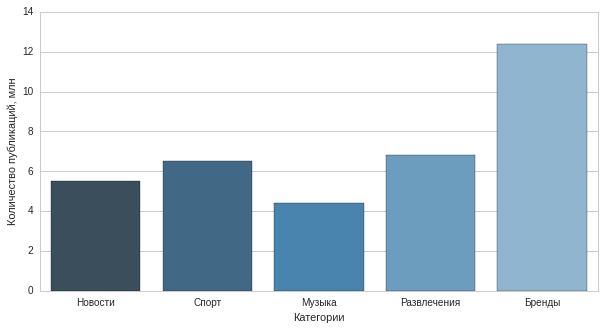
\includegraphics[width=400px]
		{imgs/NumArticles.png}
		\caption{Количество публикаций в категориях}
		\label{fig:numart}
	\end{figure} 
	
В результате  работы программного модуля для каждого сообщества был создан файл, на первой строке которого записаны идентификатор и название сообщества, а на следующих строках размещены публикации этого сообщества (на одной строке одна публикация).

	\begin{figure}
		\centering
		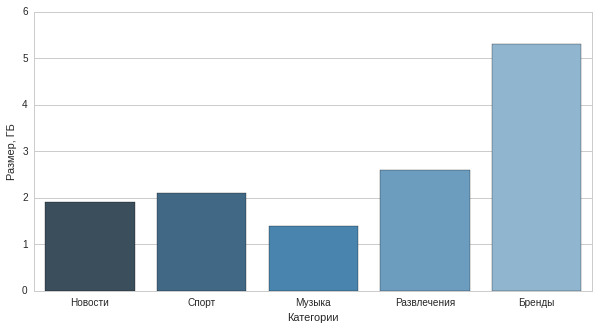
\includegraphics[width=400px]
		{imgs/SizeCat.png}
		\caption{Общий размер публикаций для каждой категории}
		\label{fig:sizecat}
	\end{figure} 
	
	
	
	
	
	
	\subsection{1.3 Предварительная обработка данных}
	Перед тем как приступить к построению тематической модели необходимо провести предварительную обработку данных. 
	Она необходима для того, чтобы избавиться от информации, которая не несет никакой смысловой нагрузки, а следовательно не оказывает заметного влияния на искомые тематики и концепции. 
	Также предварительная обработка включает в себя уменьшение числа форм слов в тексте, так как обилие различных форм слова ведет к росту словаря и снижению качества модели.
	
	В данной работе полагается, что к информации, которая не несет смысловой нагрузки относятся знаки препинания, эмотиконы \cite{bib:smiley}, гиперссылки, цифры и другие символы, не являющиеся элементами русского или английского алфавитов. К такой информации можно отнести и часто используемые слова (стоп-слова): предлоги, местоимения, союзы, числительные и частицы\cite{bib:InformationRetrieval}.
	
	Стоит заметить, что многие популярные группы часто имеют одинаковые публикации, из-за чего возникает проблема дубликатов в коллекции публикаций. В данной работе эта проблема решается с помощью хеш-функций, вычисляемых для текста каждой публикации. Хеш-функция выполняет преобразование входного массива данных в выходную битовую строку фиксированной длины \cite{bib:hash}. 
	
	
	Сокращение числа форм слов в тексте достигается путем применения стемминга или лемматизации к словам. Алгоритм стемминга заключается в поиске неизменяемой части слова, в то время как алгоритм лемматизации более сложен и необходим для поиска нормальной формы слова. Нормальной формой слова в русском языке считается: для существительных~--- единственное число, именительный падеж; для глаголов и причастий~--- глагол в форме инфинитива; для прилагательных~--- мужской род, единственное число, именительный падеж. Как правило, для предварительной обработки текста выбирается один из этих алгоритмов: для русских текстов наиболее эффективна лемматизация, для английских текстов~--- стемминг \cite{bib:Voron1}. В виду того, что в данной работе рассматриваются публикации сообществ русскоязычной социальной сети, предпочтение отдается алгоритмам лемматизации.
	
	 
	
	Для предварительной обработки данных реализован программный модуль на языке Python 2.7.
	
	Среди средств для лемматизации были рассмотрены два морфологических анализатора из программных пакетов pymorphy2 \cite{bib:pymorphy2} и pymystem3 \cite{bib:pymystem3}. Морфологические анализаторы представляют собой набор алгоритмов для сопоставления слов и их форм и выявления грамматических характристик слов. В данной работе с помощью морфологических анализаторов осуществляется приведение слов к их нормальной форме. В результате экспериментов выяснилось, что морфологический анализатор из пакета pymystem3 более эффективен, так как для определения нормальной формы слова учитываются окружающие его слова. Данный функционал отсутствует у морфологического анализатора из pymorphy2, поэтому в реализации данного программного модуля предпочтение отдано морфологическому анализатору из пакета pymystem3.
	
	Вычисление хеш-функции осуществляется с помощью встроенной функции языка Python 2.7: \textit{hash()}. Данная функция принимает на вход некоторый объект и вычисляет его хеш-значение. Стоит обратить внимание на то, что две разные строки могут иметь одинаковое значение хеш-функции. Так как вероятность такого события мала, данный эффект не окажет значительного влияния на результаты работы модуля.
	
	Для получения списка стоп-слов русского языка в программном модуле использованы пакеты nltk \cite{bib:nltk} и stop\_words \cite{bib:sw}.
	
	Работа программного модуля заключается в обработке всех файлов, полученных в разделе 1.2. В каждом файле последовательно считываются строки (текст публикации). Со всеми строками, кроме первой, выполняются следующие действия:
	
	\begin{enumerate}
	\item{ Вычисление хеш-функции; }
	\item{ Сравнение полученного значения хеш-функции строки со значениями хеш-функций ранее просмотренных строк. Если при сравнении найдутся равные значения, то данная строка удаляется из файла, иначе сохраняется значение хеш-функции и продолжается обработка строки; }
	
	\item{ Замена html-тегов в строке пробельными символами. Примеры html-тегов: <br>, <h1>. }
	
	\item{ Обработка строки морфологическим анализатором. Результатом обработки является строка, в которой все слова приведены к нормальной форме; }
	\item{ Разбиение строки по пробельному символу. Результатом разбиения будет список подстрок $L$; }
	\item{ Обработка каждой подстроки списка $L$. Результатом обработки будет список обработанных подстрок $L'$. Алгоритм обработки подстрок рассмотрен ниже;}
	\item{ Получение результирующей строки путем конкатенации подстрок списка $L'$ и пробельных символов.}
	\end{enumerate}
	
	
\begin{table}[t]
\centering
\begin{tabular}{|l|l|}
\hline
\multicolumn{1}{|c|}{\textbf{Исходный текст}}                                                                                                                                                                                             & \multicolumn{1}{c|}{\textbf{Результат обработки}}                                                                                               \\ \hline
\begin{tabular}[c]{@{}l@{}}
Андрей Кощеев и Дмитрий Головин\\ перед плей-офф  побывали в гостях \\ у воспитанников детского дома №3 \\ в рамках акции \#КлубДобрыхДел: \\
http://basket.fc-zenit.ru/photo/gl6179/\end{tabular}                    & \begin{tabular}[c]{@{}l@{}}андрей кощеев дмитрий \\ 
головин плей-офф \\ побывать гость воспитанник \\ детский дом рамка акция\end{tabular}            \\ \hline
\begin{tabular}[c]{@{}l@{}}Правозащитник Оксана Труфанова \\ рассказала {[}club27532693|"Известиям"{]} \\ 
о том, что стало причиной бунта \\
в челябинской колонии строго \\
 режима №6. \\ 
 http://izvestia.ru/news/540272\#новости\end{tabular} & \begin{tabular}[c]{@{}l@{}}правозащитник оксана \\ труфанов \\ 
 рассказывать становиться \\ 
 причина бунт челябинский \\ колония строго режим\end{tabular} \\ \hline
\begin{tabular}[c]{@{}l@{}}У нас было много театра \\ 
в последнее время. Вот теперь \\
 на музыку нажать решили. \\ 
 26 февраля, например, 
 «Сегодняночью» \\ 
 играют в клубе «J.Walker»\end{tabular}                                               & \begin{tabular}[c]{@{}l@{}}
 театр последний музыка \\ 
 нажимать решать \\ 
 февраль например \\
 сегодняночь играть клуб\end{tabular}                      \\ \hline
\begin{tabular}[c]{@{}l@{}}День матча! Единая лига ВТБ \\ 
\#ЗенитУНИКС «Сибур Арена» \\ 
15:00 (СПб) «Матч ТВ» \\ http://tickets.fc-zenit.ru/stadium.php\end{tabular}                                            & \begin{tabular}[c]{@{}l@{}}матч единый лига \\
 втб сибур арена спб матч 
\end{tabular}                                                                                                      \\ \hline


\begin{tabular}[c]{@{}l@{}} 
То прекрасное чувство, когда \\ 
распаковал новый монитор :-) \\
<br><br>Крутейший 27" LED серии 3 \\
0:) http://spr.ly/m3sv8sc\\ 
\end{tabular} 
& \begin{tabular}[c]{@{}l@{}}
 прекрасный чувство \\ 
 распаковывать новый \\
 монитор крутой \\ 
 led серия
 \end{tabular}                      \\ \hline

\end{tabular}
\caption{Пример работы программного модуля}
\label{table2}
\end{table}
	
	Алгоритм обработки подстрок, упомянутый в пункте 5, реализован в виде отдельной функции. Данной функции на вход подается строка и с ней выполняется следующая последовательность действий:
	\begin{enumerate}
	\item{ Удаление символов в начале и конце строки. Символ подлежит удалению, если он не является символом русского или английского алфавитов;}
	
	\item{ Если теперь строка содержит символы, которые не являются ни дефисом, ни символом русского или английского алфавитов, то функция возвращает пустую строку; }
	
	\item{ Распознавание аббревиатур. Строка, состоящая только из заглавных букв с длиной больше единицы и меньше семи символов распознается как аббревиатура. Если строка является аббревиатурой, то она приводится к нижнему регистру и возвращается функцией;}
	
	\item{ Если длина строки меньше трех, то функция возвращает пустую строку, иначе строка приводится к нижнему регистру; }
	
	\item{ Если строка является стоп-словом, то возвращается пустая строка, иначе возвращается сама строка.}
	\end{enumerate}
	
	Примеры работы программного модуля приведены в таблице \ref{table2} .
	

	\subsection{1.4 Результаты предварительной обработки} 
	
	В результате предварительной обработки данных число публикаций значительно уменьшилось: с 34 миллионов до 700 тысяч. Такой эффект объясняется тем, что изначально число дубликатов публикаций было довольно большим. Также предварительная обработка данных повлияла на объем необходимой памяти для хранения публикаций: общий объем занимаемой памяти уменьшился c~13~ГБ до~250~МБ.
	
	\newpage
	\section{Глава 2. Выбор и построение тематической модели}
	\subsection{2.1 Тематическое моделирование}
	\subsubsection{2.1.1 Основные сведения}
	Тематическое моделирование представляет собой  способ построения тематической модели для коллекции текстовых документов. Тематическая модель предоставляет информацию о тематиках каждого документа и о~множестве слов, образующих каждую тематику. 
	
	Тематические модели применяются в задачах тематического поиска, построения рекомендательных систем, выявления тематик и концепций в новостных потоках, а также для классификации и кластеризации документов. 
	
	В последнее время широкое распространение получили вероятностные тематические модели, которые основаны на том, что документ или термин может одновременно принадлежать разным тематикам. Вероятностная тематическая модель представляет документы в виде дискретного распределения на множестве тематик, а тематики в виде дискретного распределения на множестве терминов. Другими словами, вероятностные тематические модели выполняют <<мягкую>> кластеризацию документов и терминов по кластерам-тематикам, что решает проблему синонимии и омонимии. Слова-синонимы употребляются в одинаковых контекстах, и поэтому с высокой вероятностью принадлежат одной тематике. Слова-омонимы употребляются в различных контекстах, из-за чего распределяются в различные тематики.
	
	
	\subsubsection{2.1.2 Постановка задачи вероятностного тематического моделирования}
	
	Пусть $D$~--- множество текстовых документов, $W$~--- множество терминов, употребляемых в них. Под термином понимается либо отдельное слово, либо словосочетание. Каждый документ $d \in D$ представлен последовательностью терминов 
	$ \{w_i\}_{i=1}^{n_d}$ из $W$, где $n_d$~--- число слов в документе~$d$.
	Один и тот же термин может встречаться в документе несколько раз.
	
	Пусть $Z$~--- это конечное множесто тематик. Положим, что появление термина $w$ в каждом документе $d$ связано с некоторой, вообще говоря неизвестной, тематикой $z \in Z$. Пользуясь этим, представим множество документов в виде множества троек вида $(d,w,z)$, выбранных случайно и независмо из дискретного распределения $p(d,w,z)$, которое задано на множестве $D \times W \times Z$. Независимость элементов выборки подразумевает, что порядок терминов в документе не важен для выявления тематик. Такое предположение носит название гипотезы <<мешка слов>>.
	
	Задачу вероятностного тематического моделирования можно определить следующим образом: построить вероятностную тематическую модель для коллекции документов $D$~--- значит определить множество тематик $Z$, распределения $p(w|z)$ для всех тематик $z \in Z$ и распределения $p(z|d)$ для всех документов $d \in D$.
	
	\subsubsection{2.1.3 Порождающая вероятностная модель}

	Помимо рассмотренных выше гипотез также используется гипотеза об условной независимости, которая указывает на то, что вероятность появления термина $w$ при	условии того, что выбрана тематика $z$, описывается распределением $p(w|z)$ и не зависит от документа $d$. Это эквивалентно следующим равенствам:
	%\begin{equation}
	%	\begin{array}{c c}
			$$ p(w|d,z) = p(w|z); $$
			$$ p(d,w|z) = p(d|z)p(w|z).$$
	%	\end{array}
	%\end{equation}

	Используя гипотезу условной независимости и определения условной и полной вероятности, получаем:
	
	\begin{equation}
		p(w|d) = \sum_{z \in Z} p(w|z)p(z|d).
	\label{eq:pwd}
	\end{equation}
	
	Равенство (\ref{eq:pwd}) описывает процесс порождения множества документов $D$, если известны распределения $p(w|z)$ и  $p(z|d)$. Процесс построения тематической модели является обратной задачей и связан с поиском распределений $p(w|z)$ и  $p(z|d)$ по известному множеству документов $D$.
	
	\subsection{2.2 Выбор тематической модели}
	
	Рассмотрим две вероятностные тематические модели pLSA и LDA и сравним их. 
	Для начала введем следующие обозначения:
	
	%\begin{equation}
	$$
	\begin{array}{l l}
			
	\Phi = (\varphi_{wz})_{|W| \times |Z|}, & \quad \varphi_{wz} = p(w|z); \\
			\Theta = (\vartheta_{zd})_{|Z| \times |D|}, &  \quad
				\vartheta_{zd} = p(z|d). 
		\end{array}$$
	%	\label{eq:desc}
	%\end{equation}
	где $\Phi$~--- матрица терминов тематик, а $\Theta$ --- матрица тематик документов. Стоит обратить внимание на то, что матрицы $\Phi$ и $\Theta$ являются стохастическими. Под стохастической матрицей понимается матрица с нормированными столбцами и неотрицательными элементами.
	
	Модели pLSA и LDA основаны на вероятностной модели появления пары <<документ-слово>>,  которая может быть представлена следующим образом:
	
	\begin{equation}
	p(d,w) = \sum_{z \in Z}p(w|z) p(z|d) p(d),
	\label{eq:pmodel}
	\end{equation}
	где $p(d)$ --- это априорное распределение на множестве документов.
	
	
	
	
	
	\subsubsection{2.2.1 Вероятностное латентно-семантическое моделирование}
	\begin{figure}[h]
		\centering
		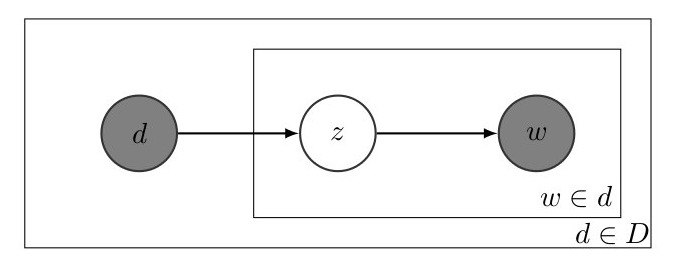
\includegraphics[width=400px]
		{imgs/PLSA.jpg}
		\caption{Байесовская сеть модели pLSA}
		\label{fig:plsa}
	\end{figure} 
	Модель pLSA можно представить в виде Байесовской сети, изображенной на рисунке \ref{fig:plsa}. Байесовская сеть представляет собой ориентированный ацикличный граф, вершины которого соответствуют случайным переменным, а ребра --- распределениям условной вероятности, где родительский узел обозначает условную переменную, а дочерний --- зависимую. Темные вершины на графе соответствуют наблюдаемым переменным (их значения известны), а белые вершины --- латентным переменным, значение которых нужно найти. В модели pLSA  $d$  и $w$ являются наблюдаемыми переменными, а $z$~--- латентной.  Прямоугольник, включающий в себя некоторый подграф $\mathbf{G}$, обозначает набор из нескольких экземпляров подграфа $\mathbf{G}$. Число экземпляров определяется надписью в правом нижнем углу прямоугольника
	\cite{bib:Heinrich}. 
	
	В pLSA для оценивания параметров по коллекции документов $D$ используется принцип максимума правдоподобия, который приводит к задаче максимизации следующего функционала (логарифма правдоподобия):
	
	\begin{equation}
		\begin{array}{c c}
		\mathcal{L}(\Phi,\Theta) = \mathlarger{ 
			\sum_{d \in D} 
			\sum_{w \in d}
			n_{dw} 
			\ln \sum_{z \in Z}
			\varphi_{wz} \vartheta_{zd} 
			\rightarrow \max_{\Phi, \Theta};
			} \\
		\mathlarger{
			\sum_{w \in W} \varphi_{wz} = 1, \quad \sum_{z \in Z} \vartheta_{zd} = 1,
		}
		\end{array}
	\label{eq:maxtask}
	\end{equation}
	где $n_{dw}$~--- это число вхождений термина $w$ в документ $d$.
	
	Обычно для решения задачи (\ref{eq:maxtask}) используется EM-алгоритм \cite{bib:Voron1}.
	%принцип работы  которого рассмотрен в приложении.
	
	Основные недостатки модели pLSA:
	\begin{itemize}
	\item{Число параметров линейно зависит от числа документов в коллекции, что ведет к переобучению модели;}
	\item{Невозможно вычислить $p(t|d)$ для документа $d$, если он добавлен в коллекцию после построения модели \cite{bib:Voron1}. }
	\end{itemize}
	
	
	\subsubsection{2.2.2 Латентное размещение Дирихле}
	
	Как и в pLSA в основе LDA лежит вероятностная модель (\ref{eq:pmodel}), но теперь делаются дополнительные предположения о том, что 
	векторы документов $\vartheta_d = (\vartheta_{dz}) \in \mathbb{R}^{|T|}$ 
	и 
	векторы тематик $\varphi_z = (\varphi_{wz}) \in \mathbb{R}^{|W|}$ 
	порождаются распределениями Дирихле с параметрами 
	$ \alpha \in \mathbb{R}^{|T|} $ 
	и
	$ \beta \in \mathbb{R}^{|W|} $ соответственно:
	
	$$  \mathlarger{
		\text{Dir}(\vartheta_d; \alpha) = 
		\dfrac
			{ \Gamma(\alpha_0)			}
			{ \prod \limits_z \Gamma (\alpha_z) }
		\prod_z \vartheta_{zd}^{\alpha_z - 1}
		},
		\alpha_z > 0, 
		\alpha_0 = \sum_z \alpha_z,
		\vartheta_{zd} > 0, 
		\sum_z \vartheta_{zd} = 1;		
	$$
	$$  \mathlarger{
		\text{Dir}(\varphi_z; \beta) = 
		\dfrac
			{ \Gamma(\beta_0)			}
			{ \prod \limits_w \Gamma (\beta_w) }
		\prod_w \varphi_{wz}^{\beta_w - 1}
		},
		\beta_w > 0, 
		\beta_0 = \sum_w \beta_w,
		\varphi_{wz} > 0, 
		\sum_w \varphi_{wz} = 1,	
	$$
	где $\Gamma (z) $~--- гамма-функция.
	
	Учитывая данные предположения, рассмотрим Байесовскую сеть модели LDA, изображенную на рисунке \ref{fig:lda}. Параметры $\alpha$ и $\beta$ являются гиперпараметрами модели и одновременно параметрами распределения Дирихле, и, как правило, задаются до начала обучения модели. Переменная $w_{n,d}$ является наблюдаемой и представляет собой термин, стоящий на $n$-ой позиции в документе $d$. Все остальные переменные являются латентными (скрытыми).
	
	Для оценки параметров модели LDA по коллекции документов $D$ применяются вариационный Байесовский вывод, метод сэмплирования Гиббса \cite{bib:Voron1} или метод Expectation-Propagation \cite{bib:Minka}.
	
	Основной недостаток модели LDA заключается в том, что априорные распределения Дирихле не моделируют никаких особенностей языка и имеют слабые лингвистические обоснования. Они используются для того, чтобы облегчить Байесовский вывод для модели \cite{bib:Voron1}.
	
	
	
	\begin{figure}
		\centering
		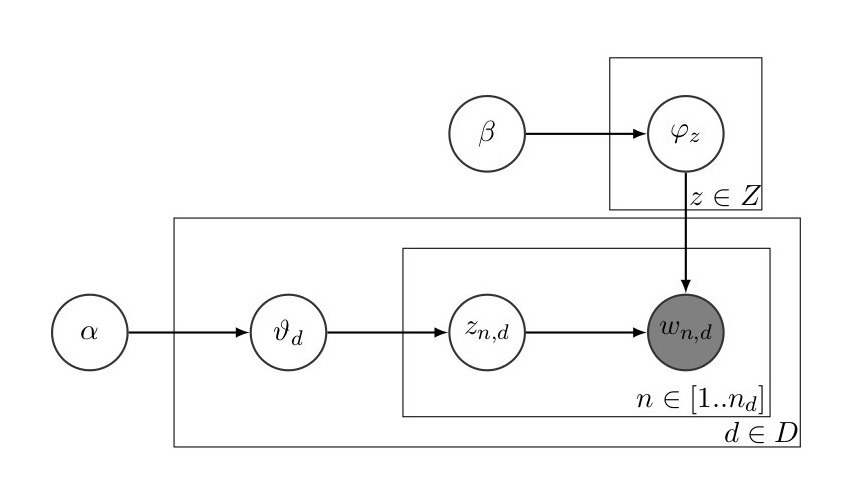
\includegraphics[width=400px]
		{imgs/LDA.jpg}
		\caption{Байесовская сеть модели LDA}
		\label{fig:lda}
	\end{figure} 
	
	
	
	
	\subsubsection{2.2.3 Вывод}
	Учитывая количество публикаций, полученных из социальных сетей, достоинства и недостатки рассмотренных моделей, разумно выбрать тематическую модель LDA. Выбор LDA облегчит работу с обучающей и тестовой выборками публикаций, так как для проверки работы модели на тестовых данных не придется выполнять построение модели заново.  Также стоит обратить внимание на то, что модель pLSA больше подвержена переобучению, чем модель LDA.
	
	В качестве метода для оценки параметров модели приоритет был отдан сэмплированию Гиббса,  так как этот метод является относительно простым и эффективным алгоритмом для решения задач статистического оценивания. Псевдокод, реализующий алгоритм сэмплирования Гиббса, приведен в приложении A.
	


	%\subsection{2.3 Реализация алгоритма построения тематической модели}
	
	%В рамках данной работы был реализова программный модуль на языке программирования Python 2.7, реализующий алгоритм построения тематической модели LDA с сэмплированием Гиббса. Псевдокод, реализующий алгоритм сэмплирования Гиббса, приведен в приложении.
	
	%Модуль поддерживает два режима работы: режим построения модели по обучающей выборке документов и режим оценивания параметров модели для тестовой выборки документов.
	
	%Для построения модели необходимо заранее определить обучающую выборку документов, количество тематик, параметры $\alpha$ и $\beta$ (параметры распределения Дирихле) и количество итераций (используются при сэмплировании Гиббса). Для оценки параметров модели тестовой коллекции необходимо задать число итераций, выполняющихся при сэмплировании Гиббса.
	
	%В любом из режимов работы модуля результатом являются матрица тематик $\Phi$, матрица документов $\Theta$, набор популярных слов для каждой тематики, привязка каждого слово каждого документа к некоторой теме.
	
	
	
	\newpage
	\section{Глава 3. Качество тематической модели}
	%\subsection{3.1 Обзор оценок качества }
	
	Одной из основных проблем тематического моделирования является оценка качества тематических моделей. 
	Это вызвано тем, что при оценивании модели нельзя ввести четкого понятия <<ошибки>>.
	Все методы оценки качества тематических моделей подразделяются на два типа: внутренние и внешние. Внутренние методы оценки дают характеристику построенной тематической модели с точки зрения исходных данных, для которых она была построена. 
	Внешние методы оценки оторажают уровень полезности тематической модели с точки зрения конечного пользователя \cite{bib:Voron1}.
	
	\subsection{3.1 Перплексия}
	
	Вычисление перплексии (perplexity) является одним из самых популярных методов внутренней оценки качества тематической модели. Перплексия отражает меру несоответствия вероятностной модели $p(w|d)$ относительно терминов $w \in d$ и определяется следующим образом:
	
	\begin{equation}
		\mathcal{P}(D) = \exp \left( - \dfrac1n \mathcal{L}(\Phi, \Theta) \right),
	\label{eq:perplexity}
	\end{equation}
	где $\mathcal{L}(\Phi, \Theta)$~--- логарифм правдоподобия, описанный в задаче (\ref{eq:maxtask}), а значение $n = \sum_{d \in D} n_d $ обозначает общее число терминов в коллекции.
	
	Маленькие значения перплекскии говорят о хорошей предсказательной способности вероятностной модели $p(w|d)$ для терминов $w$ в документе $d \in D$ \cite{bib:Heinrich}.
	
	Несмотря на свою популярность, перплексия имеет существенный недостаток, связанный с плохой интерпретируемостью числовых значений. Также важно, что перплексия зависит не только от качества построенной модели, но и от других параметров: мощность словаря, длина документов.
	
	В тематическом моделировании различают перплексию обучающей и тестовой выборок.
	Значения перплексии обучающей выборки (\ref{eq:perplexity}) являются оптимистично заниженными оценками качества модели. 
	Для того чтобы оценить обобщающую способность модели, вычисляется перплексия на тестовой выборке, минус которой выражается в чувствительности к новым словам \cite{bib:Voron1}.
	
	\subsection{3.2 Экспертная оценка}
	Экспертная оценка относится к методам внешней оценки качества тематической модели. Для каждой тематики составляется список терминов, которые наиболее популярны в ней.  Далее эти списки передаются экспертам или асессорам, и для каждой тематики они определяют ее интерпретируемость и осмысленность. Задача экспертов заключается в классификации предоставленных им тематик на два класса: тематики, которым можно дать осмысленное название и которым его дать нельзя.
	
	\subsection{3.3 Когерентность}
	
	Так как экспертная оценка является затратной операцией, были разработаны методы автоматической оценки когерентности (согласованности) тематик.
	
	Тематика называется когерентной, если наиболее встречающиеся в ней термины неслучайно часто встречаются рядом в документах коллекции.
	
	Оценка когерентности модели выполняется с помощью поточечной взаимной информации (pointwise mutual information, PMI) \cite{bib:Newman}:
	
	\begin{equation}
		PMI(z) = \mathlarger{
			\sum_{i=1}^{k-1} \sum_{j=i}^{k} \log 
			\dfrac
			{E(w_i,w_j)}
			{E(w_i)E(w_j)}
		},
	\label{eq:coherence}
	\end{equation}
	где $w_i$ --- $i$-ый термин в порядке убывания в $\varphi_{wz}$, $E(w)$ --- число документов, содержащих слово $w$, $E(w_i,w_j)$ указывает на количество документов, в которых хотя бы раз слова $w_i$ и $w_j$ встречаются рядом. Число $k$ указывает на количество рассматриваемых терминов в $\varphi_{wz}$ и обычно устанавливается равным 10 \cite{bib:Voron1}.
	
	Среднее значение когерентности для всех тематик дает хорошую оценку интерпретируемости модели \cite{bib:Newman}. Чем выше среднее значение когерентности, тем лучше согласованы темы. Преимуществом когерентности над другими методами внутреннего оценивания тематических моделей является высокая корреляция с оценками экспертов.
	
	
	\subsection{3.4 Характеристики ядер тем}
	
	
	Ядром $\mathcal{J}_z$ тематики $z$ называется множество терминов, имеющих высокую условную вероятность $p(z|w)$ для данной тематики:
	$$ \mathcal{J}_z = \{ w \in W | p(z|w) > 0.3 \}. $$
	
	Ядро используется для получения следующих мер интерпретируемости тематики $z$:
	\begin{itemize}
	\item{Чистота тематики: $purity(z) = \mathlarger \sum_{w \in \mathcal{J}_z} p(w|z)$};
	\item{Контрастность тематики: $ contrast (z) = \frac{1}{|\mathcal{J}_z|}
		\mathlarger \sum \limits_{w \in \mathcal{J}_z} p(z|w)
	$}.
	\end{itemize}
	
	Чем больше показатели чистоты и контрастности, тем лучше интерпретируема тематика.
	
	%\subsection{3.2 Оценка качества построенной тематической модели}
	
	\section{Глава 4. Эксперименты}
	
	Для проведения экспериментов с моделью LDA реализован программный модуль на языке программирования C++. Задача данного модуля по заданной обучающей выборке и выбранным параметрам построить тематическую модель LDA. Для оценки параметров модели используется алгоритм сэмплирования Гиббса, псевдокод которого приведен в приложении~A. 
	Перед построением модели указывается следующий набор параметров:
	\begin{itemize}
		\item{количество тематик;     }
		\item{гиперпараметр $\alpha$; }
		\item{гиперпараметр $\beta$;  }
		\item{число итераций для сэмплирования Гиббса.	  }
	\end{itemize}
	
	
	
	По окончании построения модели доступны матрица тематик $\Phi$, матрица документов $\Theta$ и информация о тематике для каждого термина каждого документа. Также для каждой тематики доступно множество терминов, наиболее характеризующих ее.
	
	\subsection{4.1 Обучающая и тестовая выборки}
	
	Рассмотрим тексты публикаций сообществ, полученных в результате предварительной обработки, рассмотренной в разделе 1.3. Если выражаться в терминах тематического моделирования, каждая такая публикация является документом. Объединим все публикации всех имеющихся сообществ в одно множество; назовем это множество коллекцией документов.
	
	Имеющуюся коллекцию документов необходимо разбить на две части: обучающую и тестовую выборки.
	Обучающая выборка используется для оценки параметров $\Phi$ и $\Theta$ во время обучения тематической модели.
	 Тестовая выборка необходима для оценки обобщающей способности построенной тематической модели. 
	 Не существует определенного правила для выбора пропорций разбиения коллекции документов. В работе \cite{bib:Voron1} указывается, что наиболее эффективно разбиение в отношении 9:1, где наибольшей частью является обучающая выборка.
	
	В данной работе рассматривается разбиение коллекции документов на обучающую и тестовую выборки тремя различными способами: в отношениях 4:1, 9:1 и 14:1.  Для удобства последующего изложения обучающую и тестовую выборки в соотношении 4:1 обозначим $D_A$ и $D_A'$, в соотношении 9:1~--- $D_B$ и $D_B'$, в соотношении 14:1~--- $D_C$ и $D_C'$. Получение обучающей и тестовой выборок является результатом случайного разбиения коллекции документов в соответствующих пропорциях. 
	
	Рассматриваемая коллекция состоит из 706007 документов. Размеры обучающих и тестовых выборок, полученных в результате разбиений, описанных выше, представлены в таблице \ref{traintesttable}.
	\newline
	
	
	\begin{table}[h]
\centering
\begin{tabular}{|c|c|c|}
\hline
\multicolumn{1}{|l|}{\textbf{Тип разбиения}} & \textbf{\begin{tabular}[c]{@{}c@{}}Размер \\ обучающей выборки\end{tabular}} & \textbf{\begin{tabular}[c]{@{}c@{}}Размер \\ тестовой выборки\end{tabular}} \\ \hline
4:1                                          & 564836                                                                       & 141241                                                                      \\ \hline
9:1                                          & 635409                                                                       & 70688                                                                       \\ \hline
14:1                                         & 658896                                                                       & 47181                                                                       \\ \hline
\end{tabular}
\caption{Размер обучающей и тестовой выборок для каждого типа разбиения}
\label{traintesttable}
\end{table}
	

	
	
	
	\subsection{4.1 Пример обучения тематической модели}
	
	В данном разделе построим тематическую модель для обучающей выборки документов $D_B$ и рассмотрим примеры тематик, выделенных данной моделью. Для обучения модели выбраны следующие параметры: число тематик --- 10, $\alpha$ = 0.1, $\beta$ = 0.1, число итераций --- 2000. Далее для обучения всех моделей используется 2000 итераций.
	Время обучения данной модели составило около 14 часов.
	 
	В таблице \ref{topics} представлены 10 самых характерных терминов для каждой тематики.  Из таблицы видно, что некоторым тематикам  можно дать осмысленное название, например, тематика 1 --- <<Дети>>, 3 --- <<Спорт>>, 7 --- <<Спорт>>, 8 --- <<Власть>> или <<Политика>>, 9 --- <<Культура>>. В тематиках 2, 4, 5, 6 термины также связаны между собой, но дать определенное название тематике несколько сложнее.  Тематика 0 характеризуется терминами, которые не позволяют однозначно ее интерпретировать. 
	
\begin{table}[h]
\centering
\begin{tabular}{|c|c|}
\hline
\textbf{\begin{tabular}[c]{@{}c@{}}Номер\\ тематики\end{tabular}} & \textbf{Термины}                                                                                                                        \\ \hline
0                                                                 & \begin{tabular}[c]{@{}c@{}}
свой   
самый   
друг  
знать   
ребенок \\  
говорить   
становиться   
новый   
слово   
хороший
\end{tabular}                \\ \hline
1                                                                 & \begin{tabular}[c]{@{}c@{}}
девочка   
	ребенок   
	месяц   
	давать   
	делать \\  
	малыш   
	врач   
	подсказывать   
	спать   
	ночь
\end{tabular}              \\ \hline
2                                                                 & \begin{tabular}[c]{@{}c@{}}
подсказывать   
	добрый   
	заказ   
	здравствовать   
	сайт   
	размер \\   
	заказывать   
	икеа   
	цвет   
	товар
\end{tabular}            \\ \hline
3                                                                 & \begin{tabular}[c]{@{}c@{}}
матч   
	цска   
	команда   
	клуб   
	игра \\  
	россия   
	сборная   
	футбол   
	чемпионат   
	тренер 
\end{tabular}                   \\ \hline
4                                                                 & \begin{tabular}[c]{@{}c@{}}фильм   
	конкурс   
	свой   
	новый   
	самый \\  
	получать   
	друг   
	хороший   
	победитель   
	становиться
	\end{tabular}        \\ \hline
5                                                                 & \begin{tabular}[c]{@{}c@{}}новый   
	компания   
	свой   
	получать   
	рубль  \\  
	работа   
	приложение   
	сайт   
	сеть   
	телефон\end{tabular}     \\ \hline
6                                                                 & \begin{tabular}[c]{@{}c@{}}город   
	москва   
	видео
	место   
	россия \\  
	область   
	самолет   
	дом   
	читать  
	житель\end{tabular}                     \\ \hline
7                                                                 & \begin{tabular}[c]{@{}c@{}}россия   
	матч   
	чемпионат  
	мир   
	спорт \\  
	игра   
	сборная   
	команда  
	олимпийский   
	российский \end{tabular} \\ \hline
8                                                                 & \begin{tabular}[c]{@{}c@{}}россия   
	читать   
	российский   
	далее   
	страна \\  
	украина   
	президент   
	сша   
	заявлять   
	путин  \end{tabular}           \\ \hline
9                                                                 & \begin{tabular}[c]{@{}c@{}}концерт   
	группа   
	билет   
	новый   
	песня  \\  
	фестиваль   
	самый   
	петербург   
	свой   
	театр \end{tabular}              \\ \hline
\end{tabular}
\caption{Тематики}
\label{topics}
\end{table}
	
	\newpage
	\subsection{4.2 Перплексия}
	
	В рамках данного раздела были проведены эксперименты для выявления зависимости перплексии от количества тематик и значения гиперпараметра модели $\alpha$. 
	
	Рассмотрим как влияет увеличение числа тематик модели на значение перплексии. Для этого обучим несколько моделей, гиперпараметры которых фиксированы: $\alpha =0.1$, $\beta =0.1$. На рисунке \ref{fig:PerpTopicsOnTrain} изображены графики зависимости значений перплексии обучающей выборки от количества тематик. 
	
	\begin{figure}[h]
		
		\centering
		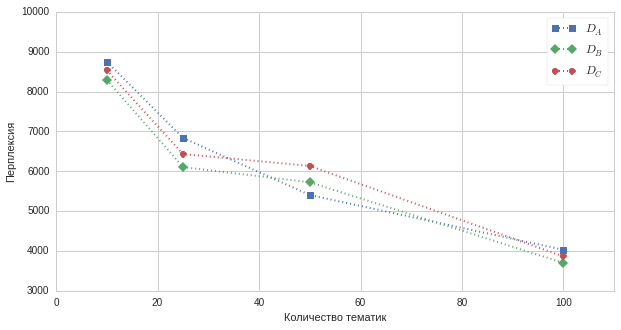
\includegraphics[width=400px]
		{imgs/PerplexityTopicsOnTrain.png}
		\caption{Зависимость перплексии обучающей выборки от количества тематик}
		\label{fig:PerpTopicsOnTrain}
	\end{figure}
	
	 На рисунке видно, что увеличение количества тематик уменьшает значение перплексии независимо от того, в каком соотношении выполнялось разбиение на обучающую и тестовую выборки.
	
	 На рисунке \ref{fig:PerpTopicsOnTest} изображены аналогичные графики, но только для перплексии тестовой выборки. Опять же значения перплексии уменьшаются при увеличении количества тематик. Стоит обратить внимание на то, что значения перплексии тестовой выборки больше значений перплексии обучающей выборки для одного и того же количества тематик. Данный эффект связан с переобучением тематической модели.
	 
	 \begin{figure}[h]
		\centering
		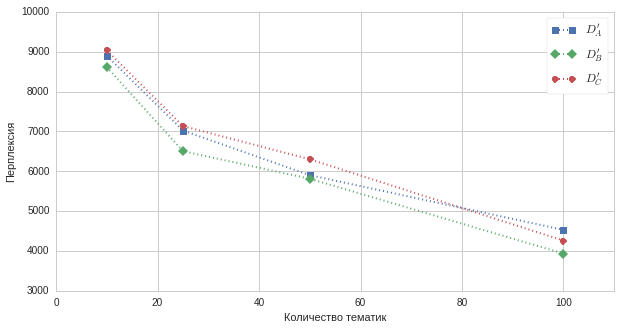
\includegraphics[width=400px]
		{imgs/PerplexityTopicsOnTest.png}
		\caption{Зависимость перплексии тестовой выборки от количества тематик}
		\label{fig:PerpTopicsOnTest}
	\end{figure}
	 
	 
	 
	 Теперь рассмотрим влияние гиперпараметра $\alpha$ на значение перплексии. Обучим тематические модели с различными параметрами $\alpha$ и с фиксированными числом тематик, равным 100, и гиперпараметром $\beta=0.1$. 
	 
	 На рисунке \ref{fig:PerpAlphaOnTrain} представлены графики зависимости перплексиии обучающей выборки от значения гиперпараметра $\alpha$, из которых видно, что уменьшение гиперпараметра $\alpha$ влечет уменьшение значения перплексиии обучающей выборки.
	 
	 \begin{figure}[h]
		\centering
		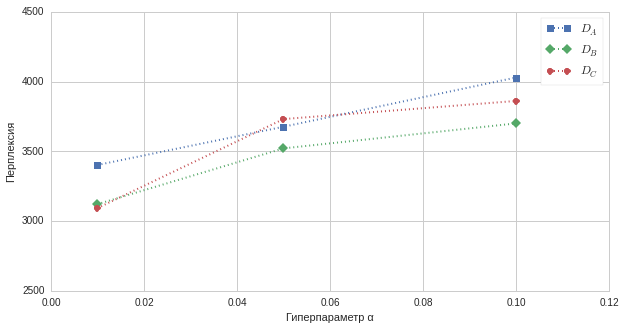
\includegraphics[width=400px]
		{imgs/PerplexityAlphaOnTrain.png}
		\caption{Зависимость перплексии обучающей выборки от гиперпараметра $\alpha$ }
		\label{fig:PerpAlphaOnTrain}
	\end{figure}
	 
	 Зависимость перплексии тестовой выборки от гиперпараметра $\alpha$, изораженная на рисунке \ref{fig:PerpAlphaOnTest}, прослеживается аналогично предыдущему примеру. Опять же заметим, что перплексия тестовой выборки превышает по показателям перплексию обучающей выборки. 
	 
	 \begin{figure}[h]
		\centering
		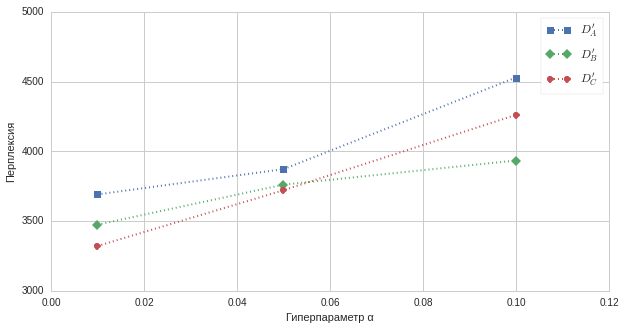
\includegraphics[width=400px]
		{imgs/PerplexityAlphaOnTest.png}
		\caption{Зависимость перплексии тестовой выборки от гиперпараметра $\alpha$ }
		\label{fig:PerpAlphaOnTest}
	\end{figure}
	 
	Проанализировав предложенные графики зависимости перплексии от параметров, можно заметить, что наихудшие значения перплексии достигаются на тематической модели, для которой разбиение на обучающую и тестовую выборки выполнялось в отношении 4:1. 
	 
	\subsection{4.3 Когерентность}
	
	В данном разделе рассмотрим зависимость среднего значения когерентности для всех тематик модели от количества тематик. Из раздела 3.3 известно, что чем выше среднее значение когерентности, тем лучше согласованы тематики.
	
	\begin{figure}[h]
		\centering
		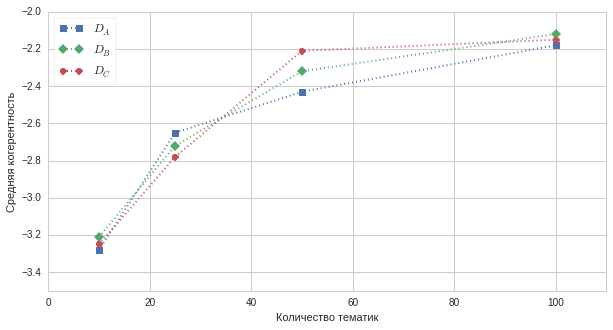
\includegraphics[width=400px]
		{imgs/CoherenceTopic.png}
		\caption{ Зависимость средней когерентности от количества тематик }
		\label{fig:coherence}
	\end{figure}
	
	На рисунке \ref{fig:coherence} представлены графики зависимости средней когерентности от количества тематик. Результаты, представленные на рисунке, говорят о том, что увеличение числа тематик влечет их лучшую согласованность.
	
	 \subsection{4.4 Результаты} 
	 
	 В разделе 4.1 был рассмотрен пример тематической модели, которая уже неплохо определяла тематики для обучающей коллекции документов. Далее был проведен ряд экспериментов для выяснения влияния параметров тематической модели на ее перплексию и среднюю когерентность. В результате проведенных экспериментов выяснилось, что модели, построенные по выборкам $D_B$ и $D_C$, имеют лучшее качество по сравнению с моделями, обученными по выборке $D_A$. 
	 
	 Из все построенных в ходе экспериментов тематических моделей наилучшее качество имела модель, построенная на обучающей выборке $D_C$ со следующими параметрами: число тематик --- 100, $\alpha = 0.01$, $\beta=0.1$. 
	 
	 
	 
	
	
	
	
	
	
	

	
		

	
	\newpage
	\section{Анализ результатов}
	%Выводы
	
	В результате проделанной работы удалось выполнить все поставленные задачи. В качестве источника данных для контекстной обработки рассматривалось множество социальных сетей, среди которых была выбрана социальная сеть VKontakte. В качестве данных для последующей обработки были выбраны публикации в  сообществах данной социальной сети. Далее были описаны методы загрузки и предварительной обработки данных. 
	Для того чтобы реализовать контекстную обработку данных были рассмотрены основные идеи тематического моделирования, а также две тематические модели: pLSA и LDA. Для дальнейшей обработки данных была выбрана модель LDA с оцениванием параметров методом сэмплирования Гиббса. 
	
	В ходе проведенных экспериментов сравнивались различные стратегии разбиения исходной коллекции на обучающую и тестовую выборки, в ходе которых выяснилось, что разбиения в соотношении 9:1 и 14:1 эффективнее разбиения 4:1
	
	
	
	
	

\begin{table}[h]
\centering
\begin{tabular}{|c|c|}
\hline
\textbf{\begin{tabular}[c]{@{}c@{}}Номер\\ тематики\end{tabular}} & \textbf{Термины}                                                                                                                        \\ \hline
5                                                                 & \begin{tabular}[c]{@{}c@{}}
россия   
	украина   
	страна   
	президент   
	сша  
	путин \\  
	москва   
	глава   
	владимир 
	власть
\end{tabular}                \\ \hline
21                                                                 & \begin{tabular}[c]{@{}c@{}}
девочка   
	ребенок   
	врач   
	малыш   
	помогать  
	мама   \\
	сын   
	говорить  
	добрый   
	ребеночек
\end{tabular}              \\ \hline
25                                                                 & \begin{tabular}[c]{@{}c@{}}
заказ  
	заказывать   
	размер   
	приходить   
	почта \\   
	получать   
	отправлять   
	посылка   
	возврат    
	доставка 
\end{tabular}            \\ \hline
46                                                                 & \begin{tabular}[c]{@{}c@{}}
матч   
	цска   
	команда   
	клуб   
	игра \\  
	россия   
	сборная   
	футбол   
	чемпионат   
	тренер 
\end{tabular}                   \\ \hline
53                                                                 & \begin{tabular}[c]{@{}c@{}}фильм   
	фильм   
	город   
	история   
	парк   
	театр \\  
	петербург   
	kudago   
	место   
	музей   
	выставка  
	\end{tabular}        \\ \hline
61                                                                 & \begin{tabular}[c]{@{}c@{}}новый   
	хороший   
	получать
   	конкурс
	победитель   
	ждать  \\
	становиться   
	участник   
	приз  
	участие	
	поздравлять\end{tabular}     \\ \hline
63                                                                 & \begin{tabular}[c]{@{}c@{}}город   
	друг   
	ребенок   
	любить  
	рука   
	женщина \\  
	слово   
	помогать   
	давать   
	понимать   
	жить   \end{tabular}                     \\ \hline

78                                                                 & \begin{tabular}[c]{@{}c@{}}россия   
	матч   
	цска   
	команда  
	клуб   
	игра \\  
	россия  
	сборная   
	чемпионат   
	футбол   
	тренер  \end{tabular}           \\ \hline

\end{tabular}
\caption{Тематики}
\label{topics1}
\end{table}
	
Также в ходе проведенных экспериментов была построена тематическая модель LDA, которая неплохо определила основные тематики. Заметим, что изначально публикации были выбраны из сообществ следующих категорий: <<Новости>>, <<Спорт>>, <<Музыка>>, <<Развлечения>>, <<Бренды>>. Из тематик, которые были определены в ходе обучения модели, явно выделяются тематики о спорте, культуре и политике. Можно отметить наличие связей между полученными тематиками и категориями сообществ.
	
	
Следующим шагом выполнялось сравнение построенной модели с другими моделями на основе таких оценок качества как перплексия и когерентность. В ходе этих экспериментов выяснилась зависимость качества модели от количества тематик и от значений гиперпараметра $\alpha$. В результате проведенных экспериментов среди всех построенных тематических моделей была выбрана модель с наилучшей оценкой качества. В таблице \ref{topics1} приведены наборы терминов для некоторых тематик, выделенных этой моделью. Среди тематик, представленных в таблице, выделяются тематики о власти, детях, спорте, культуре и другие.
	
Основываясь на результатах работы построенной тематической модели, можно сделать вывод, что методы тематического моделирования хорошо проявляют себя при контекстной обработке данных.





 


	
	
	
	\newpage
	\section{Заключение}
	
	В рамках данной работы было рассмотрено применение вероятностных тематических моделей для контекстной обработки данных, полученных из сообществ социальной сети VKontakte в виде текстов публикаций. Для достижения этой цели были реализованы алгоритмы для загрузки данных из социальной сети, предварительной обработки данных и построения тематической модели LDA. В ходе экспериментов была проведена оценка качества нескольких тематических моделей, среди которых была выбрана модель с лучшими оценками качества. Также эксперименты показали зависимость качества модели от количества тематик и ее гиперпараметров.	
	
	 В результате экспериментов выяснилось, что модель LDA хорошо справляется с задачей выделения ключевых тематик и концепций в коллекции документов, а значит применима для контекстной обработки данных.
	
	Для дальнейших исследований имеет смысл рассмотреть робастные тематические модели и методы аддитивной регуляризации тематических моделей. Робастные модели основываются на том, что на появление отдельных терминов в документе влияет не только тематика документа, но также фон и шум. К фону, как правило, относятся стоп-слова, которые не удалось отбросить на стадии предварительной предобработки. К шуму относятся термины, характерные для конкретного документа. Методы аддитивной регуляризации позволяют создавать большое число разнообразных тематических моделей, не прибегая к вероятностным допущениям, как это было сделано в модели LDA. 
	
	
	
	\newpage
	\section{Список литературы}
	
    \begingroup
    \let\clearpage\relax
    \vskip-3cm
	\begin{thebibliography}{9}
	
		\bibitem{bib:Kaklauskas}
		Arturas Kaklauskas Biometric and Intelligent Decision Making Support. Springer, 2015. 220~p.
		
		\bibitem{bib:InformationRetrieval}
		Christopher D. Manning, Prabhakar Raghavan, Hinrich Schütze Introduction to Information Retrieval. Cambridge University Press, 2008. 506~p.
		
		\bibitem{bib:Hoffman}
		Thomas Hofmann Probabilistic latent semantic indexing //
		Proceedings of the 22nd annual international ACM SIGIR conference on Research and development in information retrieval, 1999. P.~50~--~57.
		
		\bibitem{bib:Blei}
		David Blei, Andrew Y. Ng, Michael I. Jordan Latent Dirichlet Allocation // Journal of Machine Learning Research 3, 2003. P.~993~--~1022.
		
		\bibitem{bib:Blei2}
		David Blei Introduction to Probabilistic Topic Models.  Communications of the ACM, 2012. P.~77~--~84.
		
		\bibitem{bib:Heinrich}
		Gregor Heinrich Parameter estimation for text analysis. Technical
report. Fraunhofer IGD, Darmstadt, Germany, 2005.

		

		\bibitem{bib:Voron1}
		Воронцов К.В. Вероятностное тематическое моделирование. Москва, 2013.

		\bibitem{bib:Popularity}
		Number of global social network users 2010-2019.  http://www.statista.com/statistics/278414/number-of-worldwide-social-network-users/
		
		\bibitem{bib:PopularNetwork}
		Global social networks ranked by number of users 2016. http://www.statista.com/statistics/272014/global-social-networks-ranked-by-number-of-users/
		
		\bibitem{bib:vkapi}
		API VKontakte. https://vk.com/dev/apiusage
		
		\bibitem{bib:methods}
		Методы API VKontakte. https://vk.com/dev/methods

\bibitem{bib:smiley}
		Эмотикон. https://ru.wikipedia.org/wiki/Эмотикон
		
		\bibitem{bib:hash}
		Хеш-функция. https://ru.wikipedia.org/wiki/Хеширование
		
		\bibitem{bib:pymorphy2}
		Документация морфологического анализатора pymorphy2. https://pymorphy2.readthedocs.io/en/latest/
	
		\bibitem{bib:pymystem3}
		Документация pymystem3. https://pypi.python.org/pypi/pymystem3/0.1.1
		
		\bibitem{bib:nltk}
		Документация nltk. 
		http://www.nltk.org/
		
		\bibitem{bib:sw}
		Документация stop\_words
		https://pypi.python.org/pypi/stop-words
		
		\bibitem{bib:Minka}
		Thomas Minka Expectation Propagation for Approximate Bayesian Inference //
		Proceedings of the 17th Conference in Uncertainty in Artificial Intelligence. University of Washington, Seattle, Washington, USA, 2001. P.~362~--~369.
		
		
		\bibitem{bib:Newman}
		Newman D., Lau J. H., Grieser K., Baldwin T. 
		Automatic evaluation of topic coherence // 
		Human Language Technologies: The 2010 Annual Conference of the
North American Chapter of the Association for Computational Linguistics. HLT
’10. Stroudsburg, PA, USA: Association for Computational Linguistics, 2010. P.~100~--~108.
		
	
	\end{thebibliography}
    \endgroup
    
	\section{Приложение A}
	\subsubsection{Псевдокод алгоритма сэмплирования Гиббса}
	
	\begin{algorithm}[H]
		\SetAlgoLined
		\KwData{ коллекция документов D; число тематик |Z|; параметры $\alpha$ и $\beta$}
		\KwResult{ Распределения $\Phi$ и $\Theta$ }
		$ n_{wz}, n_{zd}, n_z, n_d := 0 $ для всех $d \in D, w \in W, z \in Z$; \\
		\ForEach{ $i := 1,...,i_{\max}$}{
			\ForEach{ $d \in D$ } {
				\ForEach{ $w_1,...,w_{n_d} \in d$ }{
					\If{$ i > 1 $}{ 
						z := $z_{dw}$; $n_{wz} := n_{wz} - 1$; 
						$n_{zd} := n_{zd} - 1$; \\
						$n_z := n_z - 1$; $n_d := n_d - 1$;
					}
					$p(z|d,w) = \text{norm}_{z \in Z} \left( 
					\dfrac{n_{wz} + \beta_w}{n_z + \beta_0} 
					\cdot
					\dfrac{n_{zd} + \alpha_z}{n_d + \alpha_0} 
					\right)$ для всех $ z \in Z$; \\
					сэмплировать одну тематику z из распределения $p(z|d,w)$; \\
					$z_{dw} := z$;
					$n_{wz} := n_{wz} + 1$,;
					$n_{zd} := n_{zd} + 1$;
					$n_z := n_z + 1$; $n_d := n_d + 1$;
				}
			}
		}
		$\varphi_{wz} := \frac{n_{wz}}{n_z} $ для всех $w \in W, z \in Z$; \\
		$\vartheta_{zd} := \frac{n_{zd}}{n_d} $ для всех $d \in D, z \in Z$;
		
		
		
		
\end{algorithm}
	
	
	
	
	%%Приложи сюда свой код	
\end{document}